%!TEX root = main.tex

\section{Kapitel 6: Module und Datenkapseln\hfill}
\label{sec:Kapitel 6: Module und Datenkapseln}

\subsection{Modul (Unit)\hfill}
\label{sec:Modul (Unit)}

\subsubsection{Motivation\hfill}
\label{sec:Motivation}
\begin{itemize}
	\item \textbf{Arbeitsteilung}
	\item[\-] Grosse Programme werden von mehreren Personen entwickelt. Praktikabel ist, wenn nur eine Person an einer bestimmten Datei arbeitet.
	\item \textbf{Effizienz}
	\item[\-] Eine Übersetzungseinheit (Datei) muss bei jeder Änderung neu übersetzt werden (je grösser die Datei desto langsamer die Übersetzung)
	\item \textbf{Strukturierung}
	\item[\-] Ein grosses  Programm in mehrere vernünftige Teile (Baugruppen, Units) aufteilen (Divide and conquer)
\end{itemize}

\subsubsection{Nomenklatur: Modul vs. Unit\hfill}
\label{sec:Nomenklatur: Modul vs. Unit}
\begin{itemize}
	\item Ein Programmbaustein wird traditionell mit Modul (der oder das Modul) bezeichnet
	\item Der Test eines Moduls heisst folglich Modultest
	\item Das Vorgehen, welches Module generiert, heisst Modularisierung
	\item Heute üblicher wird Modul mit Unit, der Test mit Unittest bezeichnet, das Vorgehen heisst weiterhin Modularisierung
	\item Prinzipiell spreche ich künftig meist von Unit und Unittest
\end{itemize}

\subsubsection{Ziele der Modularisierung\hfill}
\label{sec:Ziele der Modularisierung}
\begin{itemize}
	\item Klare, möglichst schlanke Schnittstellen definieren
	\item Units so bilden, dass Zusammengehörendes in einer Unit isoliert wird (Kohäsion) soll hoch sein
	\item Schnittstellen zwischen den Units sollen klein sein (Kopplung soll klein sein)
	\item Abhängigkeiten unter den Units sollen eine Hierarchie bilden, zirkuläre (gegenseitige) Abhängigkeiten müssen vermieden werden
\end{itemize}

\subsubsection{Eigenschaften einer Unit (eines Moduls)\hfill}
\label{sec:Eigenschaften einer Unit (eines Moduls)}
\begin{itemize}
	\item realisiert eine in sich abgeschlossene Aufgabe
	\item kommuniziert über ihre Schnittstelle mit der Umgebung
	\item kann ohne Kenntnisse ihres inneren Verhaltens in ein Gesamtsystem integriert werden
	\item ihre Korrektheit kann ohne Kenntnis ihrer Einbettung in einem Gesamtsystem nachgewiesen werden (mittels Unittest)
\end{itemize}

\subsubsection{Bestandteile eine C++-Programms\hfill}
\label{sec:Bestandteile eine C++-Programms}
\begin{itemize}
	\item \textbf{Eine} Hauptfunktion main()
	\item Eine Reihe von unabhängigen Programmbausteinen (Units)
\end{itemize}

\subsubsection{Unitkonzept\hfill}
\label{sec:Unitkonzept}
\begin{itemize}
	\item Interface definiert die Schnittstelle, d.h. die Deklarationen wie Funktionsprototypen, etc. (Schaufenster)
	\item Implementation: In diesem Teil sind die Unterprogramme definiert, d.h. auscodiert (Werkstatt)
	\item Das Interface wird in einer Headerdatei (*.h) beschrieben, die Implementation liegt in einer *.cpp-Datei
\end{itemize}
\noindent
\begin{figure}[hh]
	\centering
	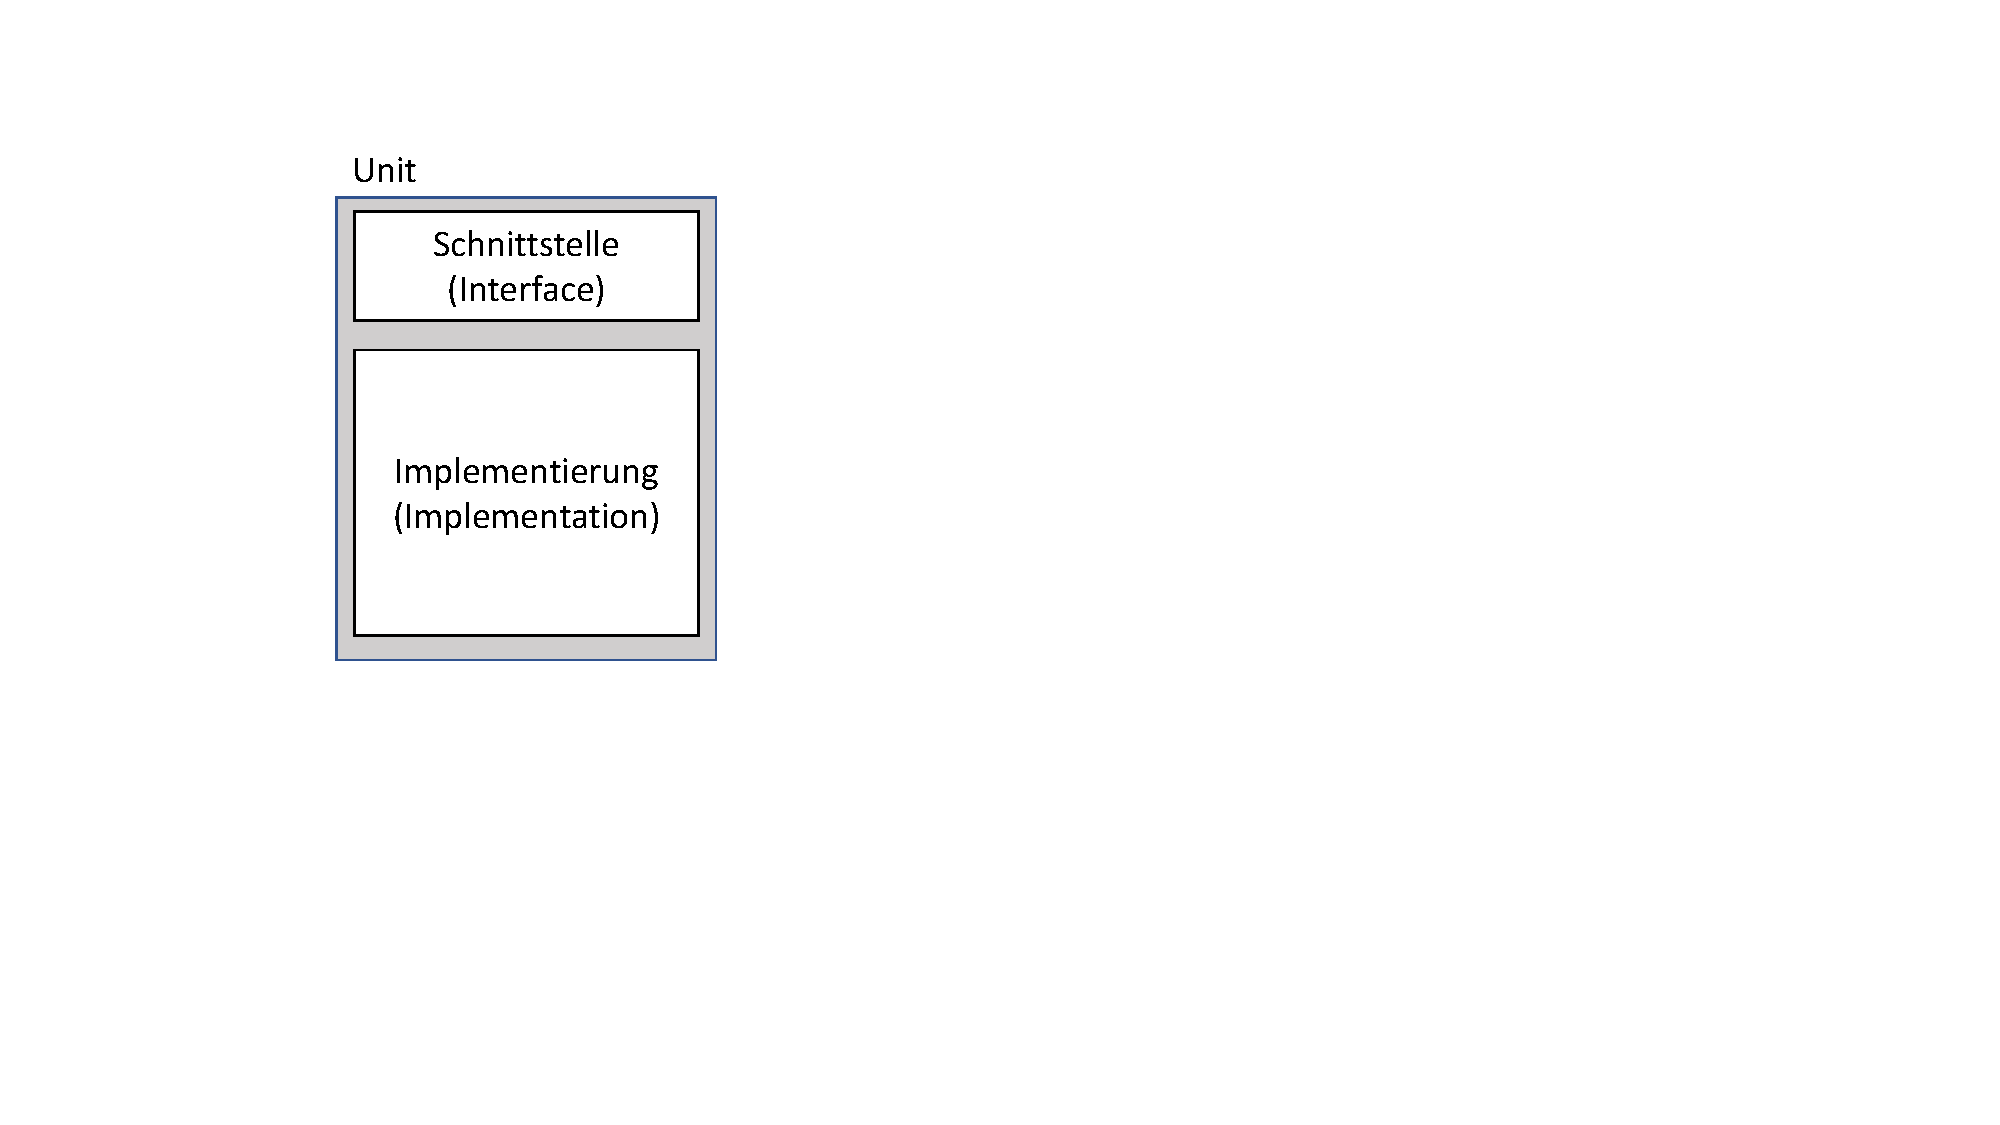
\includegraphics[width=0.3\linewidth]{unit1.pdf}
\end{figure}

\subsection{Geheimnisprinpzip (Information Hiding)\hfill}
\label{sec:Geheimnisprinzip (Information Hiding)}

\subsubsection{Information Hiding\hfill}
\label{sec:Information Hiding}
\begin{itemize}
	\item In der Schnittstelle (Headerdatei) wird alles beschrieben, was ein Nutzer dieser Unit wissen muss
	\item Der innere Aufbau der Unit (*.cpp) muss (darf) dem Nutzer der Unit nicht bekannt sein, er benötigt diese Informationen auch gar nicht
	\item Der Nutzer der Unit darf keine Annahmen bezüglich des inneren Aufbaus der Unit treffen
	\item Der Entwickler der Unit darf den inneren Aufbau der Unit ändern, solange dadurch die Schnittstelle nicht geändert werden muss
\end{itemize}

\subsubsection{Konzept der Datenkapsel\hfill}
\label{sec:Konzept der Datenkapsel}
\begin{itemize}
	\item Eine Unit besteht aus Funktionen und Daten
	\item In der Schnittstelle wird definiert, was für den Nutzer zur Verfügung steht. Dies können Funktionen und Daten sein
	\item Die Datenkapsel fordert nun zusätzlich, dass auf die Daten nicht direkt zugegriffen werden darf, sondern nur über Zugriffsfunktionen
\end{itemize}

\subsubsection{Beispiel für Datenzugriff bei Datenkapsel\hfill}
\label{sec:Beispiel fuer Datenzugriff bei Datenkapsel}
\noindent
\begin{minipage}{\linewidth}
	\begin{lstlisting}
	// interne Daten
	int counter;	// gehoert zur Unit, nicht in Interface
			// wie kann das in C bewerkstelligt werden?
		
	// Schnittstelle (Interface)
	voi setCounter(int c)
	{
		counter = c;
	}
	
	int getCounter(void)
	{
		return counter;
	}
	\end{lstlisting}
\end{minipage}

\subsubsection{Beispiel für Unit Rechteck (ohne Datenkapsel)\hfill}
\label{sec:Beispiel fuer Unit Rechteck (ohne Datenkapsel)}
\noindent
\begin{minipage}{\linewidth}
	\begin{lstlisting}
	// interne Daten
	double a;	// 1. Seite
	double b;	// 2. Seite
	double area;	// Rechtecksflaeche
	
	// Schnittstelle (Interface)
	
	// direkter Zugriff auf a, b, area
	// Annahme: area hat immer den aktuellen Wert, d.h. es muss
	// bei jeder Aenderung von a und b (durch den Client!) berechnet werden
	\end{lstlisting}
\end{minipage}
\begin{achtung}
	Sehr gefährlich! (kann kaum sichergestellt werden)
\end{achtung}

\subsubsection{Beispiel für Unit Rechteck: Verbesserung \#1}
\label{sec:Beispiel fuer Unit Rechteck: Verbesserung 1}
\noindent
\begin{minipage}{\linewidth}
	\begin{lstlisting}
	// interne Daten
	double a;	// 1. Seite
	double b;	// 2. Seite
	double area;	// Rechtecksflaeche
	
	// Schnittstelle (Interface)
	// kein direkter Zugriff mehr auf a, b, area
	// Funktionen setA(), setB(), getA(), getB(), getArea()
	void setA(double newA)
	{
		a = newA;
		area = a * b;
	}
	
	double getArea(void)
	{
		return area;
	}
	\end{lstlisting}
\end{minipage}
\begin{hinweis}
	Evtl. gefährlich (Berechnung von area könnte vergessen werden). Und: soll die Multiplikation wirklich bei jeder Aenderung durchgefuehrt werden?
\end{hinweis}

\subsubsection{Beispiel für Unit Rechteck: Verbesserung \#2}
\label{sec:Beispiel fuer Unit Rechteck: Verbesserung 2}
\noindent
\begin{minipage}{\linewidth}
	\begin{lstlisting}
	// interne Daten
	double a;	// 1. Seite
	double b;	// 2. Seite
	// double area;	// Rechtecksflaeche, Attribut wird entfernt
	
	// Schnittstelle (Interface)
	// Attribut area wird entfernt
	// Funktionen setA(), setB(), getA(), getB(), getArea()
	void setA(double newA)
	{
	a = newA;
	}
	
	double getArea(void)
	{
		return a * b;
	}
	\end{lstlisting}
\end{minipage}
\begin{hinweis}
	Dank Datenkapsel darf das Attribut area entfernt werden. Die Schnittstelle ändert sich dadurch nicht.
\end{hinweis}

\subsubsection{Unit nutzen\hfill}
\label{sec:Unit nutzen}
\noindent
\begin{minipage}{\linewidth}
	\begin{lstlisting}
	#include "foo.h"
	// dadurch wird die Schnittstelle der Unit foo bekanntgemacht
	\end{lstlisting}
\end{minipage}

\subsubsection{Unit-Schnittstelle definieren (in Headerdatei)\hfill}
\label{sec:Unit-Schnittstelle definieren}
\noindent
\begin{minipage}{\linewidth}
	\begin{lstlisting}
	// Datei: foo.h
	#ifndef FOO_H_
	#define FOO_H_
	
	// Deklarationen
	
	
	#endif /* FOO_H_ */
	\end{lstlisting}
\end{minipage}
\begin{hinweis}
include-Guard: verhindert das mehrfache include derselben Datei
\end{hinweis}

\subsubsection{Deklarationsreihenfolge in der Headerdatei (*.h)\hfill}
\label{sec:Deklarationsreihenfolge in der Headerdatei}
\begin{achtung}
	kein using namespace ... in Headerdateien!
\end{achtung}
\begin{enumerate}
	\item Dateikommentar
	\item \#include der verwendeten System-Header (iostream, etc.)
	\item[\-] \#include <...>
	\item \#include der projektbezogenen Header (\#include "...")
	\item Konstantendefinitionen
	\item typedefs und Definitionen von Strukturen
	\item Allenfalls extern-Deklarationen von globalen Variablen
	\item Funktionsprototypen, inkl. Kommentare der Schnittstelle, bzw. Klassendeklarationen
\end{enumerate}
\begin{hinweis}
	Punkte 2-7 sind innerhalb des inlcude-Guards.
\end{hinweis}

\subsubsection{Reihenfolge in der Implementierungsdatei (*.cpp)\hfill}
\label{sec:Reihenfolge in der Implementierungsdatei}
\begin{enumerate}
	\item Dateikommentar
	\item \#include der verwendeten System-Header (iostream, etc.)
	\item \#include der projektbezogenen Header
	\item allenfalls globale Variablen und statische Variablen
	\item Präprozessor-Direktiven
	\item Funktionsprototypen von lokalen, internen Funktionen
	\item Definition von Funktionen und Klassen
	\item[\-] \color{\ownRed} (Kommentare aus Headerdatei nicht wiederholen!)
\end{enumerate}

\subsubsection{\#include-Konzept}
\label{sec:include-Konzept}
\begin{itemize}
	\item Mit den \#includes wird oft ein Riesenchaos veranstaltet
	\item Der "Einfachheit halber" werden ab und zu einfach alle oder fast alle Headerdateien inkludiert
	\item Das muss unbedingt verhindert werden
\end{itemize}
\textbf{Regel: In jeder Datei (*.h, *.cpp, *.c) werden genau die Headerdateien inkludiert, welche diese Datei selbst benötigt!}

\subsubsection{Unit compilieren\hfill}
\label{sec:Unit compilieren}
\begin{center}
	\textbf{g++ \color{\ownRed}-c\color{black} foo.cpp}
\end{center}
\begin{itemize}
	\item Dadurch entsteht noch kein ausführbares Programm, sondern nur die Datei foo.o, der Objectcode
	\item Dies muss mit allen *.cpp-Dateien gemacht werden
\end{itemize}

\subsubsection{Units linken\hfill}
\label{sec:Units linken}
\begin{center}
	g++ -o foo foo.o goo.o hoo.o
\end{center}
\begin{itemize}
	\item Alle Objectdateien müssen gelinkt werden
	\item Dadurch werden allenfalls noch offene Verbindungen (Links) zu aufgerufenen Funktionen aufgelöst
\end{itemize}

\subsubsection{Buildprozess\hfill}
\label{sec:Buildprozess}
\begin{itemize}
	\item Der Buildprozess beinhaltet alle Schritte, um ein ausführbares Programm zu erhalten, bzw. aufzubauen (englisch to build)
	\item[\-] g++ -c foo.cpp
	\item[\-] g++ -c goo.cpp
	\item[\-] g++ -c hoo.cpp	
	\item[\-] g++ -o foo foo.o goo.o hoo.o
\end{itemize}
\begin{hinweis}
	Es wäre mühsam, wenn diese Befehle jedesmal neu eingetippt werden müssten. Deshalb wird in der Praxis oft ein Buildtool eingesetzt, z.B. make.
\end{hinweis}

\subsection{Make-Tool}
\label{sec:Makt-Tool}

\subsubsection{Abhängigkeiten zwischen Dateien}
\label{sec:Abhaengigkeiten zwischen Dateien}
\noindent
\begin{figure}[hh]
	\centering
	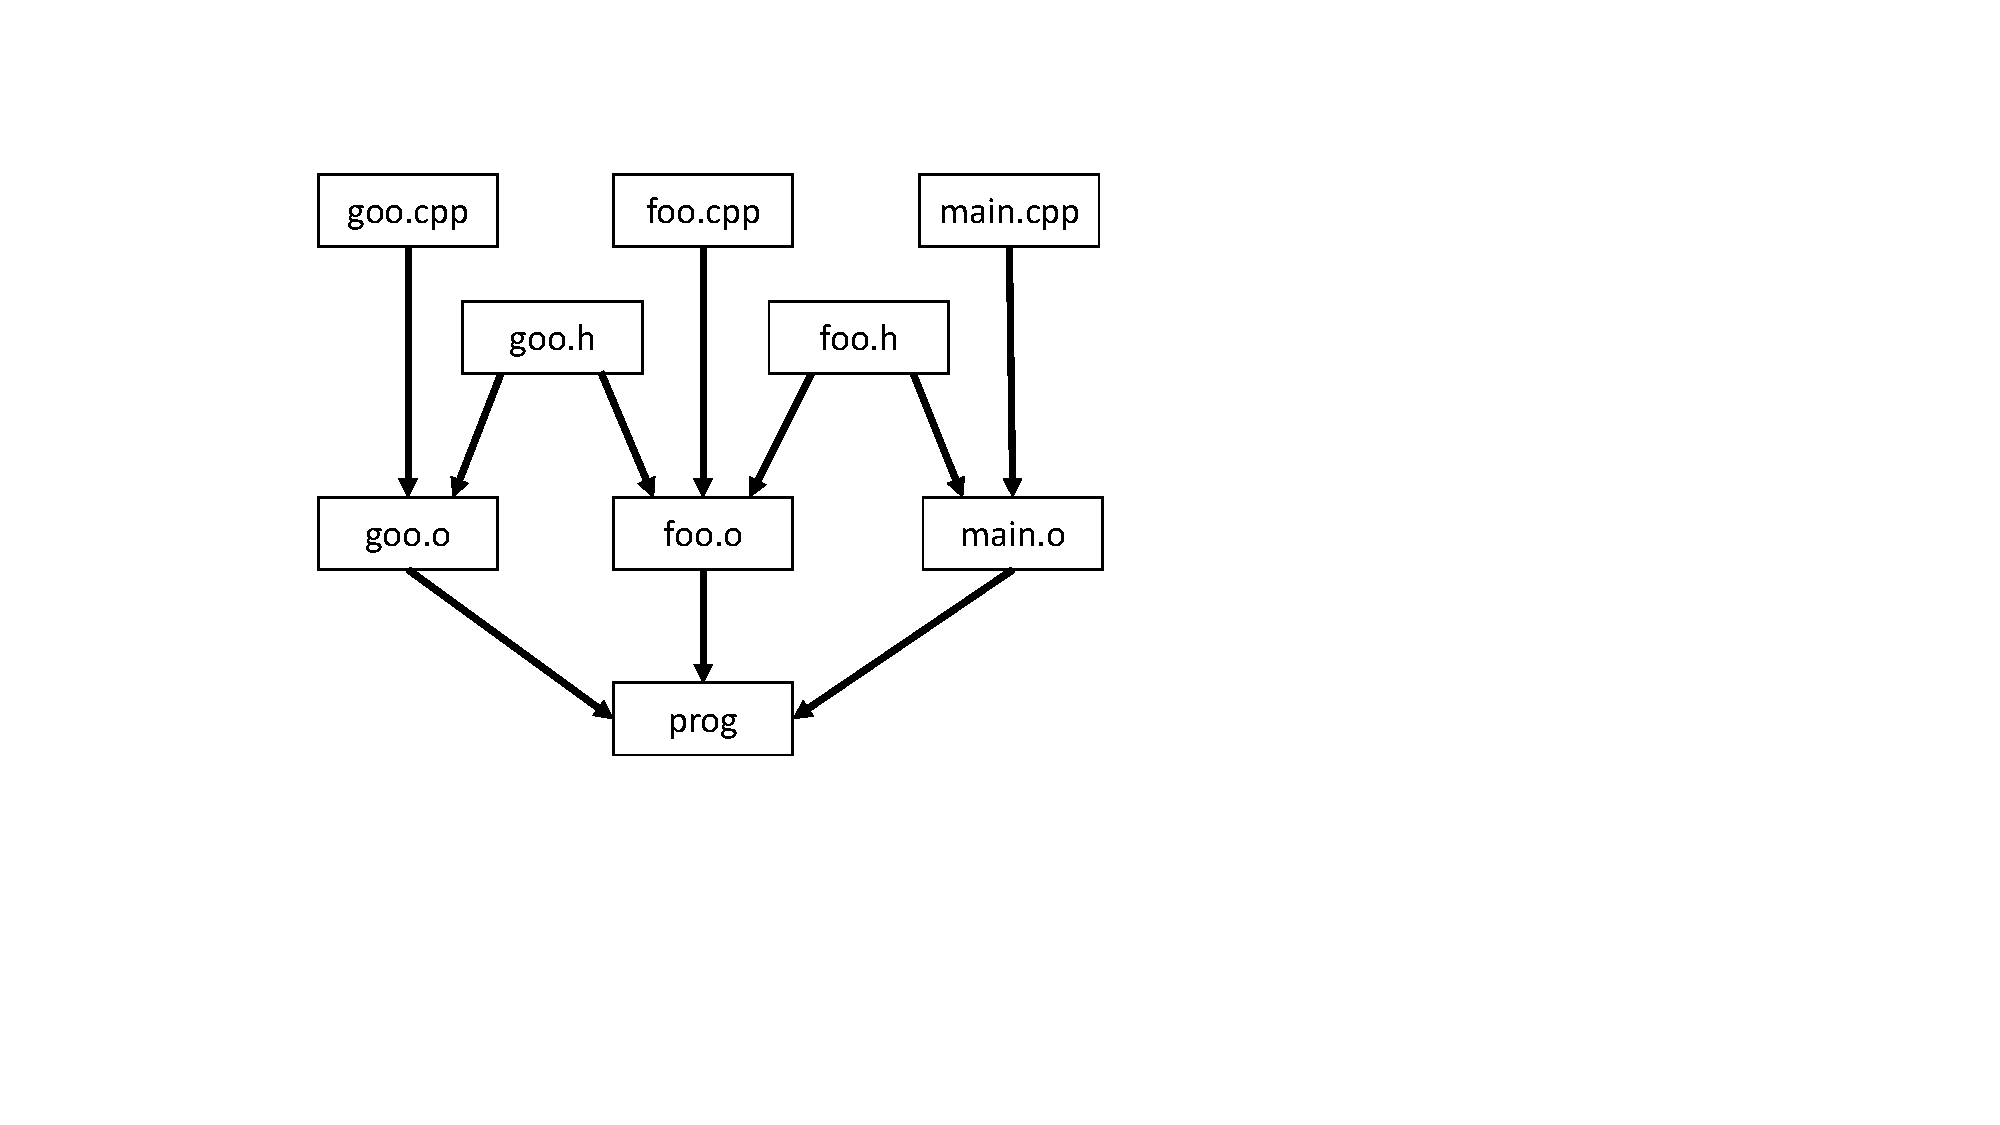
\includegraphics[width=0.5\linewidth]{make1.pdf}
\end{figure}

\subsubsection{make-File}
\label{sec:make-File}
\begin{itemize}
	\item In einem make-File können Abhängigkeiten definiert werden
	\item Wenn eine Datei geändert wurde, dann werden alle Operationen ausgeführt mit den Dateien, welche von dieser geänderten Datei abhängen
	\item Der Befehl (g++) wird z.B. nur dann ausgeführt, wenn sich an den Dateien, zu denen eine Abhängigkeit besteht, etwas geändert hat
\end{itemize}

\subsubsection{Beispiel: makefile}
\label{sec:Beispiel: makefile}
\noindent
\begin{figure}[hh]
	\centering
	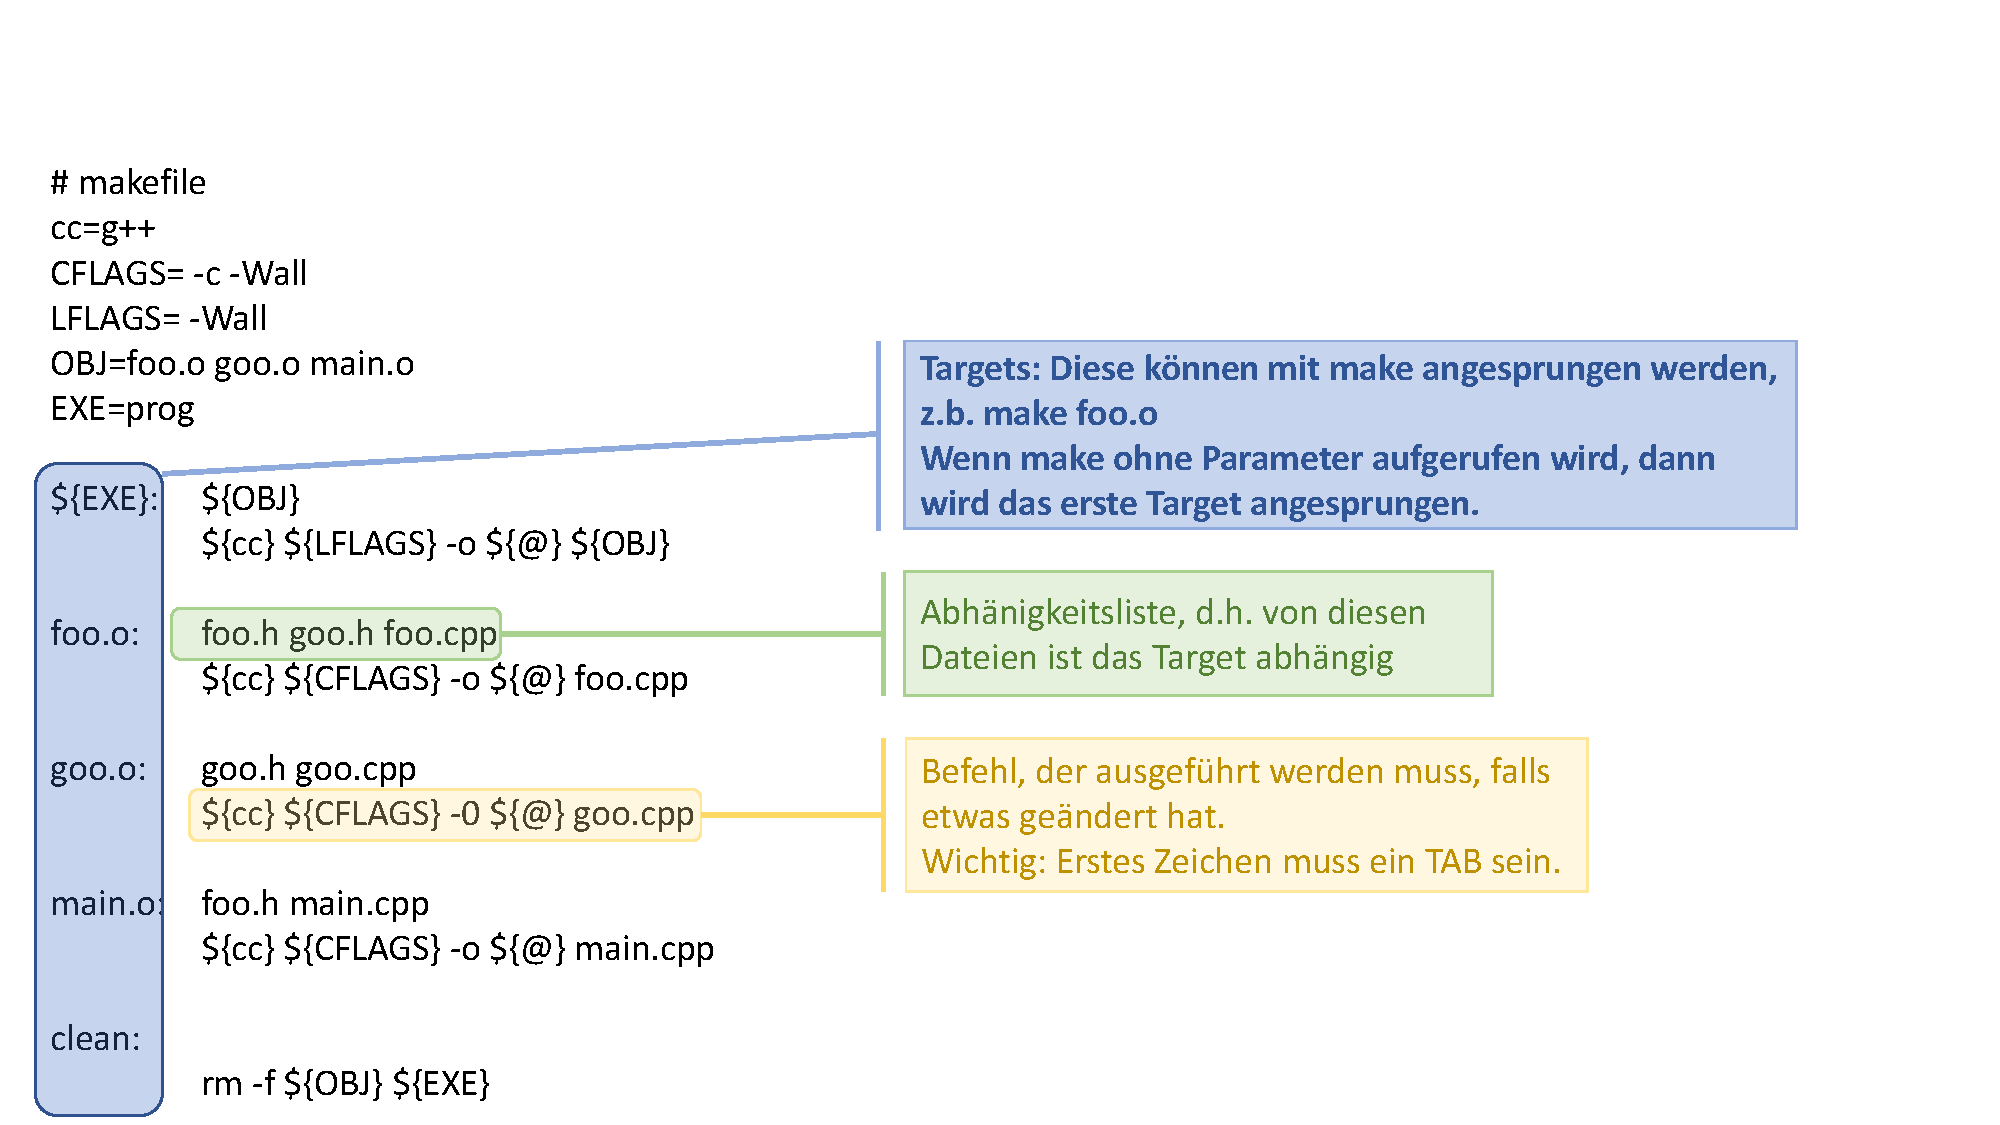
\includegraphics[width=\linewidth]{makefile.pdf}
\end{figure}